% ПРАВИЛО: фигурные скобки, которые относятся к синтаксису LaTeX, 
% следует дублировать, а фигурные скобки, относящиеся к синтаксису
% строковой интерполяции Python, нет.

\documentclass[
    11pt,
    a4paper,
    utf8,
]{article}

\usepackage{style_template}

\begin{document}

\title{ Аналитический отчет по оценке усталостной долговечности силовых элементов транспортных машин под воздействием стационарных гауссовских процессов } % заголовок отчета
\author{\itshape Иванов И.И. } % имя автора работы
\date{}
\maketitle

\thispagestyle{fancy} % задает стиль страницы

%\tableofcontents

\section{Оценка усталостной долговечности по модели J.W. Miles}

Модель Miles \cite{miles-1954}, строго говоря, применима только к узкополосным случайным процессам (процессам с узким энергетическим спектром), поэтому при нагружении широкополосными процессами модель дает слишком консервативные оценки

\begin{align}\label{eq:miles}
	Y_{NB}(s_{\sigma}) = \Big[ \, \dfrac{f}{C} \, ( \sqrt{2} s_{\sigma} )^m \, \Gamma \bigg( 1 + \dfrac{m}{2} \bigg) \, \Big]^{-1}, \ C = \sigma_{-1\text{д}}^m N_0,
\end{align}
где $ f $ -- эффективная частота случайного процесса, Гц; $ \sigma_{-1\text{д}} $ -- предел выносливости детали, МПа; $ s_{\sigma} $ -- стандартное отклонение случайного процесса, МПа; $ m $ -- тангенс угла наклона левой ветви кривой выносливости; $ \Gamma(\cdot) $ -- гамма-функция.

Усталостная долговечность по модели \eqref{eq:miles} составляет $ Y_{NB} = 9661.80 $, сек.

\section{Оценка усталостной долговечности по модели P.H. Wirsching и C.L.~Light}

Модель Wirsching-Light \cite{wirshing-light-1980} это один из вариантов коррекции модели J.W. Miles \eqref{eq:miles}. В случае строго узкополосного процесса, т.е. когда $ \alpha_2 = 1 $, оценки по рассматриваемой модели и по модели Miles совпадают $ Y_{WL}(\varepsilon = 0 ,s_{\sigma}) = Y_{NB}(s_{\sigma})$
\begin{gather}\label{eq:wirsching-light}
	Y_{WL}(s_{\sigma}) = \chi_{WL}^{-1} \, Y_{NB}(s_\sigma), \\
	\chi_{WL} = a_0(m) + [\, 1 - a_0(m) \,]\, (1 - \varepsilon)^{ b_0(m) }, \notag \\
	a_0(m) = 0.926 - 0.033 m, \ b_0(m) = 1.587 m - 2.323, \notag \\
	\varepsilon = \sqrt{1 - \alpha_2^2}, \ \alpha_2 = \dfrac{ \lambda_2 }{ \sqrt{ \lambda_0\, \lambda_4} } \notag \\
	\underset{d = 1, 2, \ldots}{\lambda_d} = \int\limits_{0}^{+\infty} w^d\, S(w) \mathrm{d}w, \notag
\end{gather}
где $ S(w) $ -- спектральная плотность мощности процесса.

Усталостная долговечность по модели \eqref{eq:wirsching-light} составляет $ Y_{WL} = 10733.18 $, сек (см.~\pic{fig:graph}).
\begin{figure}[h!]
	\centering
	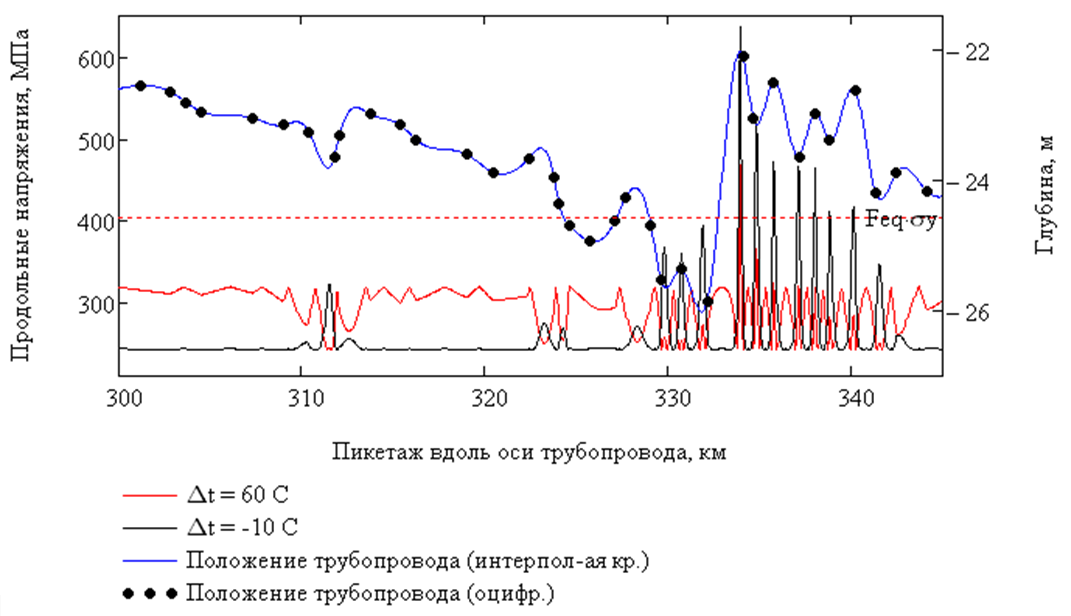
\includegraphics[scale=0.65]{figures/figure.png}
	\caption{ Распределение продольных напряжений }\label{fig:graph}
\end{figure}

\section{Оценка усталостной долговечности по модели D. Benasciutti и R.~Tovo}

Модель Tovo-Benasciutti имеет вид \cite{tovo-benasciutti-2006}
\begin{gather}\label{eq:tovo-benasciutti}
	Y_{TB}^{RFC} = \big[ b_{app} D_{NB} + (1 - b_{app}) D_{RC} \big]^{-1}, \\
	D_{RC} \approx D_{NB} \alpha_2^{m-1}, \ D_{NB} = Y_{NB}^{-1}, \notag \\
	b_{app} = [\, 1.112 \,(\, 1 + \alpha_1 \alpha_2 - (\alpha_1 + \alpha_2) \,) \, e^{2.110 \, \alpha_2} + (\alpha_1 - \alpha_2)\,] \dfrac{ \alpha_1 - \alpha_2 }{ (\alpha_2 - 1)^2}, \notag
\end{gather}
где $ D_{NB}, D_{RC} $ -- скалярные меры усталостных повреждений соответственно по модели \eqref{eq:miles} и по методу размахов.

Усталостная долговечность по модели \eqref{eq:tovo-benasciutti} составляет $ Y_{TB}^{RFC} = 9805.39 $, сек.

\appendix

\section{Листинги}

\subsection{Генератор псевдослучайного гауссовского процесса с автокорреляционной функцией экспоненциально-косинусного типа}

\begin{lstlisting}[
style = ironpython,
numbers = none	
]
def gauss_with_expcos_family_acf_base(
	*,
	a0: float,
	a1: float,
	b1: float,
	b2: float,
	N: int,
) -> np.array:
	"""
	Описание
	--------
	Опорный алгоритм построения дискретной реализации ПСП
	с КФ экспоненциально-косинусного семейства
	
	Параметры
	----------
	a0 : параметр модели ПСП.
	a1 : параметр модели ПСП.
	b1 : параметр модели ПСП.
	b2 : параметр модели ПСП.
	N : число отсчетов ПСП.
	
	Возвращает
	-------
	xi : массив элементов ПСП с заданной КФ.
	"""
	
	xi = np.zeros(N)
	# инициализация первых двух элементов массива ПСП
	# ПС числами с равномерным распределеннием
	for i in range(2):
		xi[i] = rnd.rand()
	
	# массив гауссовских ПСЧ с нулевым МО и единичной дисперсией
	x = rnd.randn(N)
	
	for n in range(1, N):
		xi[n] = a0 * x[n] + a1 * x[n - 1] + b1 * xi[n - 1] + b2 * xi[n - 2]
	
	return xi
\end{lstlisting}


\begin{thebibliography}{99}\addcontentsline{toc}{section}{Список литературы}
	\bibitem{miles-1954}{\emph{Miles J.W.} On structural fatigue under random loading // Journal Aueronaut Science. 1954. V. 21. P. 753~--~762.}
	
	\bibitem{wirshing-light-1980}{\emph{Wirsching P.H}, \emph{Light C.L.} Fatigue under wide band random processes // Journal Struct Division ASCE. 1980. V 106 (7). P. 1593 -- 1607.}
	
	\bibitem{tovo-benasciutti-2006}{\emph{Benasciutti D.}, \emph{Tovo R.} Comparison of spectral methods for fatigue analysis of broad-band Gaussian random processes // Probabilistic Engineering Mechanics. 2006. V. 21. P.287 -- 299.}
\end{thebibliography}

\end{document}